 \chapter{\uppercase{Design of Experiments}}
   \label{training}

Design of experiments (DoE) are a set of strategies that choose or allocate training point locations for a surrogate model. \emph{Training point selection} is also being termed as \emph{sampling} by many investigators, but \emph{sampling} should only refer to the process of probing the surrogate model to obtain approximated function values. This unfortunate terminology has been adopted by many investigators perhaps due to the use of many sampling techniques for training point selection (e.g. Monte Carlo sampling for random training point selection, latin hypercube sampling for pseudo-random training point selection and so on).


The location and number of training points used to construct the surrogate model  is known to have a significant effect on its accuracy.
Training point selection approaches (or DoE) can be broadly classified into domain-based and response-based approaches~\cite{Arora2007}.
In domain-based approaches, training points are chosen based on the information available from the domain (e.g. distance between two training points), whereas in response-based approaches, 
the training points are chosen based on the information provided by the surrogate model (e.g. function values, expected improvement).
Domain-based training point selection is either random or based on space-filling concepts that try to fill the domain evenly with training points.
It is, in general, not possible for the user to select the number of training points a priori to ensure a given accuracy of a surrogate due to the non-linearity of most functions of interest.
Response-based approaches enhance the efficiency of the training point selection process by using information from the existing metamodel.
This is because the user could monitor the progress of the model and choose to stop or extend the training point selection process.
The following is a brief outline of some important domain- and response-based approaches used for training point selection found in the literature.

\section{Domain-Based Approaches}
\label{domain}

\subsection{{Monte Carlo}}\label{Montecarlo}
Monte Carlo (MC) techniques~\cite{Metropolis49,Fishman96,Ecuyer2009} are perhaps the simplest of all DoE methods. Here, a random number generator is used to select training point locations in the domain. 
A major drawback of MC is that large areas of the domain may be left unexplored while others may be sampled densely~\cite{Sobol94,Keane2005,Forrester2008}.

\subsection{{Latin Hypercube}}
Latin hypercube sampling (LHS) was introduced by McKay~\etal~\cite{McKay79} for designing computer experiments as an alternative to MC sampling techniques. 
The basic idea is to divide the range of each variable into $N$ bins of equal probability, which yields $N^M$ bins in the domain, where $M$ is the dimension of the problem. 
Subsequently, $N$ training points are generated for each variable such that no two values lie in the same bin (as shown in Figure~\ref{LHSSampling}).
The LHS algorithm generates training points in a box-shaped domain as follows~\cite{Keane2005},
\beq
x^{(i)}_{j}=\dfrac{{\pi_{j}^{(i)}+U_j^{(i)}}}{N}, \quad \forall \quad 1\le{j}\le{M}, \quad 1\le{i}\le{N},
\label{LHSmath}
\eeq
where $x^{(i)}_j$ is the $j-$th component of the $i-$th training point, $U\in[0,1]$ is an uniform random number, and $\pi$ is an independent random permutation of the sequence of integers $0,1,\ldots,N-1$.
In Figure~\ref{LHSConvergence} persistent fluctuations in the accuracy (determined by the root mean square error (RMSE)) of a generic surrogate model built using LHS or MC as DoE method can be noticed.
In spite of increasing the number of training points, the RMSE does not decrease,  because all these points are picked at random.
Thus, a superior strategy for training point selection is required to ensure that the RMSE will reduce when the number of training points increase, and this has been one of the major motivations for this research.

\begin{figure}[h]
  \centering
  \begin{minipage}[b]{0.48\linewidth}
    \includegraphics[width=1.0\textwidth]{figures/latin.eps} \caption{An example of LHS in a two-dimensional domain.}
    \label{LHSSampling}
  \end{minipage}
  \begin{minipage}[b]{0.48\linewidth}
    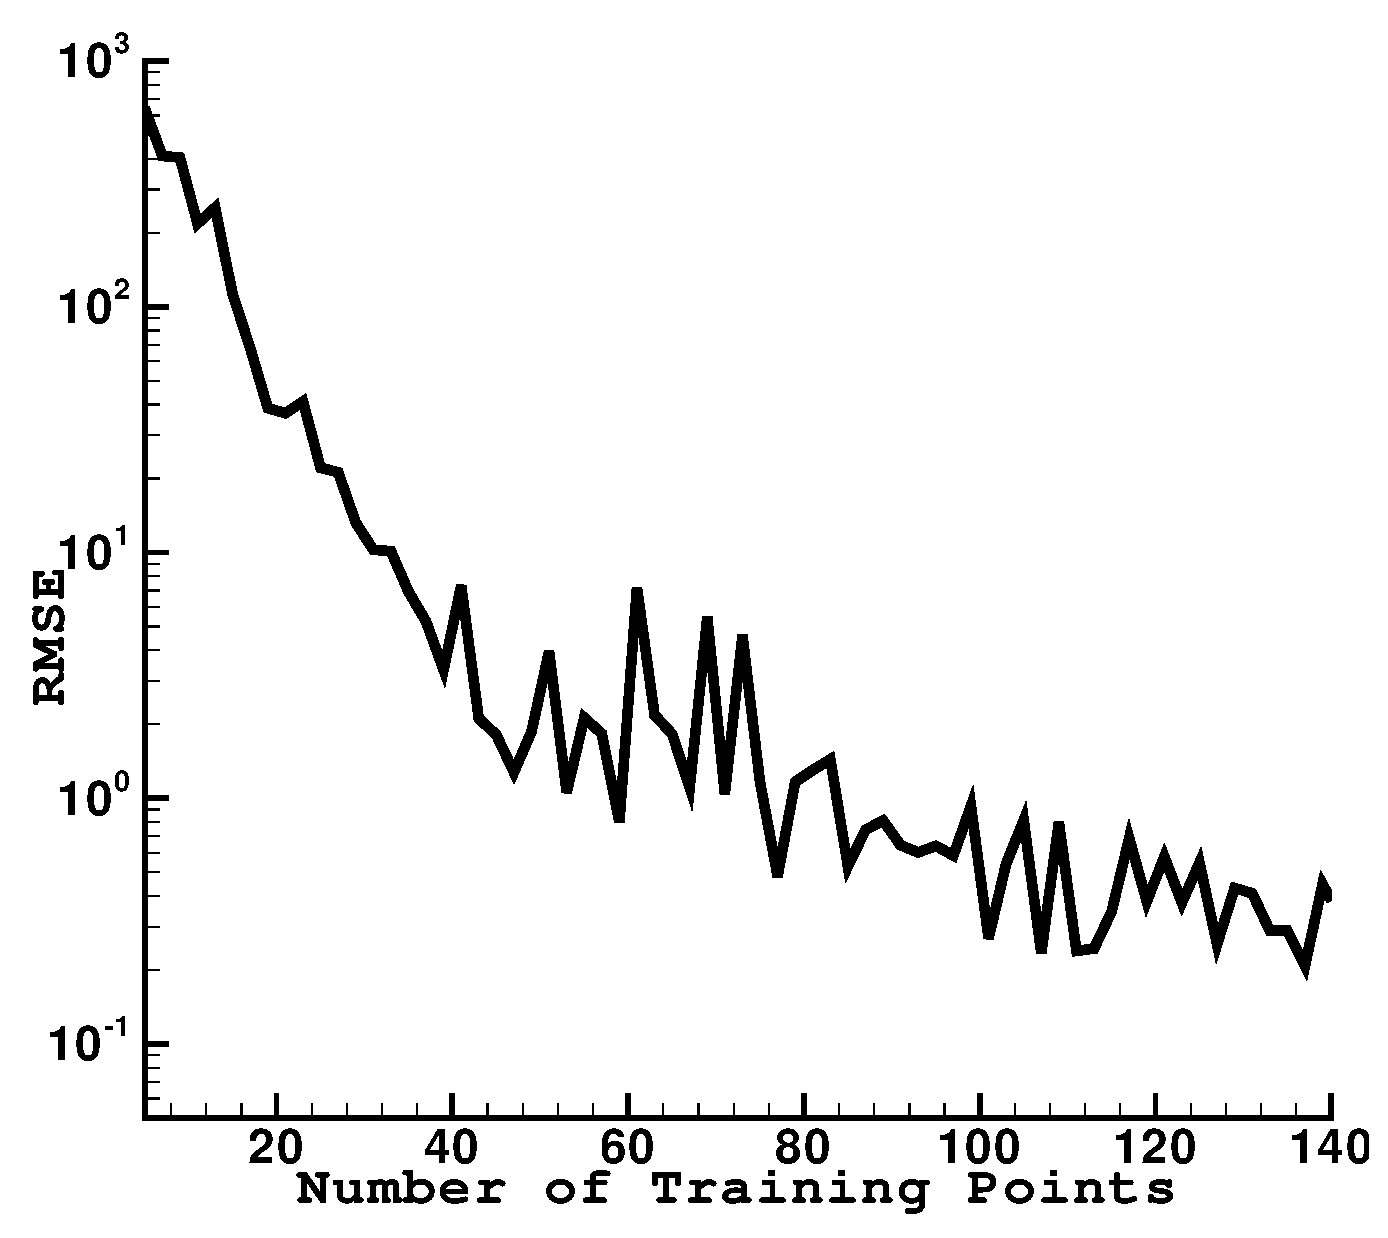
\includegraphics[width=1.0\textwidth]{figures/LHSblack.eps} \caption{Convergence history of a generic surrogate model using LHS or MC.}
  \label{LHSConvergence}
  \end{minipage}
\end{figure}

\begin{figure}[h]
  \begin{minipage}{0.48\linewidth}
    \centering
    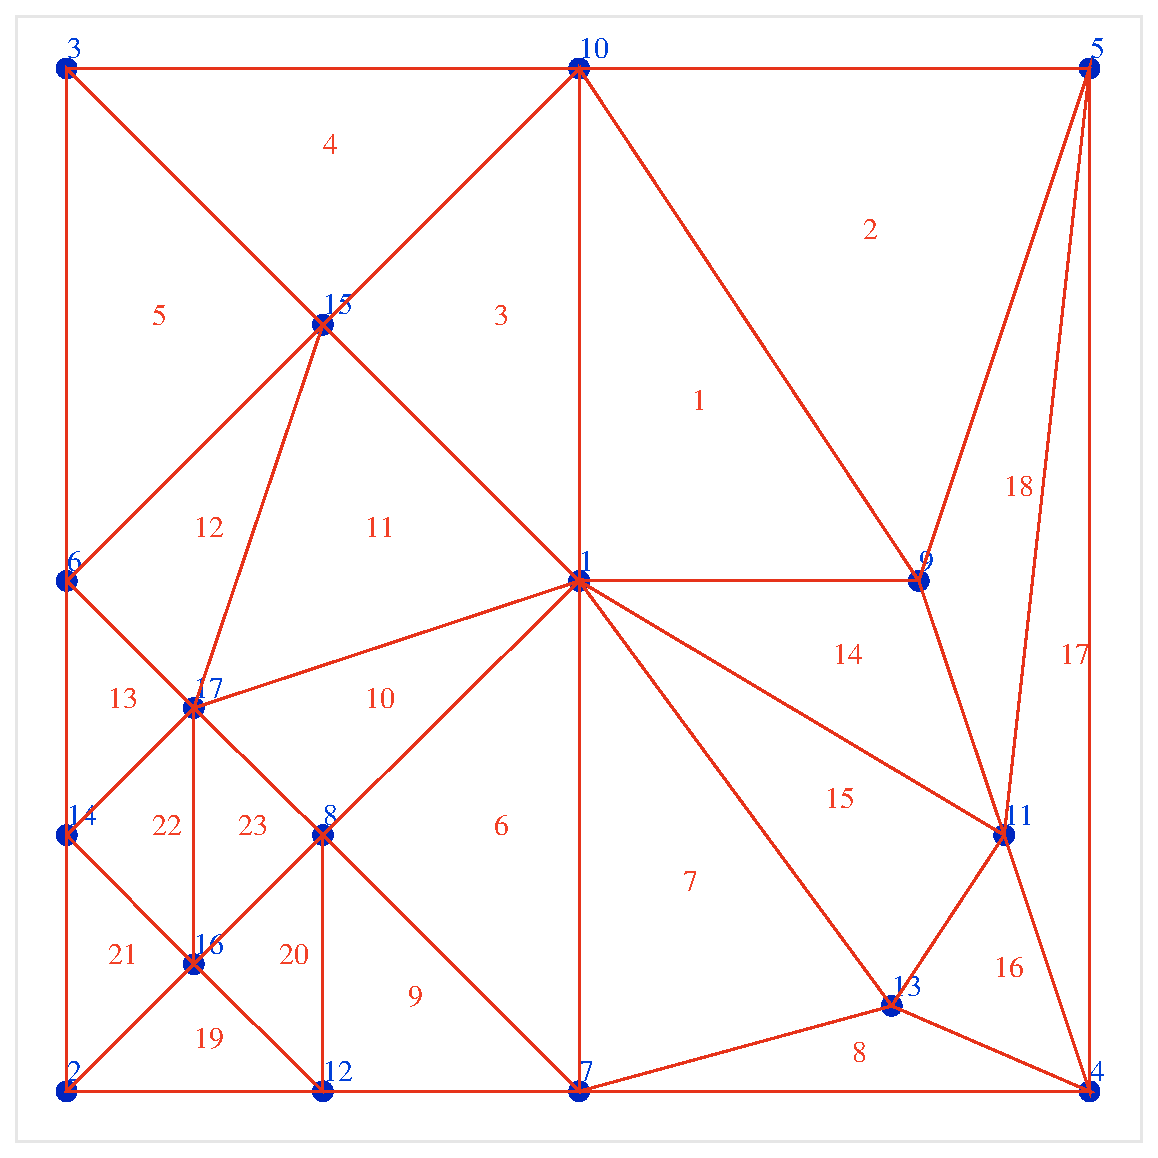
\includegraphics[width=0.95\textwidth]{figures/triangulation.eps} 
    \caption[A Delaunay triangulation schematic.]{A Delaunay triangulation schematic is shown, where points numbered 1 to 5 are the initial training points and 12 points have been added subsequently by splitting the domain into triangles.}
    \label{triangle}
  \end{minipage}
  \hfill
  \begin{minipage}{0.48\linewidth}
    \centering
    \includegraphics[width=0.95\textwidth]{figures/latinspl.eps}
    \caption{An illustration showing poor LHS distribution of training points.}
    \label{LHSspl}
  \end{minipage}%
\end{figure} 

\subsection{Delaunay Triangulation}
Delaunay triangulation is a geometrical method of training point selection, where the domain is divided into hyper-triangles and the training points are chosen at geometrical significant location such as the centers of the hyper-triangles and midpoints of the edges as shown in Figure~\ref{triangle}.
A major drawback of Delaunay triangulation is that it does not scale well to higher dimensions: the required minimum number of points become quickly large~\cite{Rumpfkeil2011a} .

\subsection{Quasi-random Sequences}
\begin{figure}[h!]
\centering
\begin{minipage}[b]{0.32\linewidth}
   \includegraphics[width=1.0\textwidth]{figures/Faure50.eps} \subcaption{Faure}
\end{minipage}
\begin{minipage}[b]{0.32\linewidth}
   \includegraphics[width=1.0\textwidth]{figures/Halton50.eps} \subcaption{Halton}
\end{minipage}
\begin{minipage}[b]{0.32\linewidth}
   \includegraphics[width=1.0\textwidth]{figures/Hammersley50.eps} \subcaption{Hammersley}
\end{minipage}
\begin{minipage}[b]{0.32\linewidth}
   \includegraphics[width=1.0\textwidth]{figures/Niederreiter50.eps} \subcaption{Niederreiter}
\end{minipage}
\begin{minipage}[b]{0.32\linewidth}
   \includegraphics[width=1.0\textwidth]{figures/Sobol50.eps} \subcaption{Sobol}
\end{minipage}
\begin{minipage}[b]{0.32\linewidth}
\includegraphics[width=1.0\textwidth]{figures/Lhs50.eps} \subcaption{Latin hypercube}
\end{minipage}
\caption[Quasi-random sequences for 50 training points.]{Training point distributions with quasi-random sequences using 50 points. A typical LHS distribution is also shown for comparison.}
\label{QMC50}
\end{figure}

Quasi-random sequences~\cite{Ecuyer2009} also known as \emph{quasi-Monte Carlo} or \emph{low discrepancy sequences} produce a sequence of deterministic points that fill the multidimensional space more uniformly than uncorrelated random points produced by pseudo-random number generators. They are primarily developed for the purpose of approximating multidimensional integrals efficiently using a better space filling than random or pseudo-random approaches such as LHS. %They are based on the calculation of discrepancy: comparison of the actual number of points present and the number of points that should be present in the multidimensional space. The discrepancy can be defined as a measure of how much the distribution of points deviate from an ideal uniform distribution. 
 Although pseudo-random numbers and quasi-random sequences both produce space filling designs, there are significant differences between the two. For a pseudo-random number generator such as LHS, it is possible for all $N$ points to coincidentally be restricted to a particular region in the domain, or a distribution such as the one shown in Figure~\ref{LHSspl} can occur. These are indeed undesirable characteristics in a training point selection strategy. It is not the case with quasi-random sequences where the points are constrained by a low-discrepancy requirement and are generated in a highly correlated manner such that the next point knows where the previous points are located. 

\begin{figure}[h!]
\centering
\begin{minipage}[b]{0.32\linewidth}
   \includegraphics[width=1.0\textwidth]{figures/Faure250.eps} \subcaption{Faure}
\end{minipage}
\begin{minipage}[b]{0.32\linewidth}
   \includegraphics[width=1.0\textwidth]{figures/Halton250.eps} \subcaption{Halton}
\end{minipage}
\begin{minipage}[b]{0.32\linewidth}
   \includegraphics[width=1.0\textwidth]{figures/Hammersley250.eps} \subcaption{Hammersley}
\end{minipage}
\begin{minipage}[b]{0.32\linewidth}
   \includegraphics[width=1.0\textwidth]{figures/Niederreiter250.eps} \subcaption{Niederreiter}
\end{minipage}
\begin{minipage}[b]{0.32\linewidth}
   \includegraphics[width=1.0\textwidth]{figures/Sobol250.eps} \subcaption{Sobol}
\end{minipage}
\begin{minipage}[b]{0.32\linewidth}
\includegraphics[width=1.0\textwidth]{figures/Lhs250.eps} \subcaption{Latin hypercube}
\end{minipage}
\caption[Quasi-random sequences for 250 training points.]{Training point distributions with quasi-random sequences using 250 points. A typical LHS distribution is also shown for comparison.}
\label{QMC250}
\end{figure} 


Figures~\ref{QMC50} and~\ref{QMC250} show typical distributions using popular quasi-random sequences such as Faure, Halton, Hammersley, Niederreiter, and Sobol~\cite{Hammersley,Sobol94,Ecuyer2009}. It can be noticed that these low discrepancy sequences fill the domain more uniformly, when compared to LHS that features a poor distribution.
Though quasi-random sequences serve well to approximate multidimensional integrals by virtue of their nice space-filling properties, they can not be expected to be a good candidate for training point selection, as they are insensitive to the function to be modeled and do not consider the response values or any form of available information from the metamodel. % This is an inefficient use of computational resources for the training of a surrogate model.


\subsection{Tensor Product and Sparse Grid Quadratures}
\begin{figure}[h]
\centering
\begin{minipage}[b]{0.32\linewidth}
   \includegraphics[width=1.0\textwidth]{figures/legord3.eps}\subcaption{Order 3}
\end{minipage}
\begin{minipage}[b]{0.32\linewidth}
   \includegraphics[width=1.0\textwidth]{figures/legord5.eps}\subcaption{Order 5}
\end{minipage}
\begin{minipage}[b]{0.32\linewidth}
   \includegraphics[width=1.0\textwidth]{figures/legord10.eps}\subcaption{Order 10}
\end{minipage}
\caption{Gauss-Legendre grid distribution in two dimensions.}
\label{legendre}
\end{figure}

Quadratures determine the nodes (training points) based on the underlying probability distribution of the random variables \emph{i.e.,} at the roots of corresponding orthogonal polynomials: Gauss-Hermite and Gauss-Legendre quadratures have their nodes distributed at the roots of Hermite and Legendre polynomials, respectively. They are also originally developed to approximate multidimensional integrals more effectively. Figure~\ref{legendre} shows an example of Gauss-Legendre quadrature with increasing order in a two-dimensional space. Multidimensional quadratures are easily obtained by tensor products of corresponding one-dimensional quadratures. Though they are shown to provide optimal convergence~\cite{Xiu2010,Knio2010}, they become computationally intractable in higher dimensions, as they require $(N+1)^M$ function evaluations in M-dimensions. 
\begin{figure}[h!]
\centering
\begin{minipage}[b]{0.32\linewidth}
   \includegraphics[width=1.0\textwidth]{figures/sparse_gl_d2_level1.eps}\subcaption{Level 1}
\end{minipage}
\begin{minipage}[b]{0.32\linewidth}
   \includegraphics[width=1.0\textwidth]{figures/sparse_gl_d2_level3.eps}\subcaption{Level 3}
\end{minipage}
\begin{minipage}[b]{0.32\linewidth}
   \includegraphics[width=1.0\textwidth]{figures/sparse_gl_d2_level5.eps}\subcaption{Level 5}
\end{minipage}
\caption{Gauss-Legendre sparse grid distribution in two dimensions.}
\label{gl_sparse}
\end{figure}
\begin{figure}[h!]
\centering
\begin{minipage}[b]{0.32\linewidth}
   \includegraphics[width=1.0\textwidth]{figures/SparseHermitedim2lev1.eps}\subcaption{Level 1}
\end{minipage}
\begin{minipage}[b]{0.32\linewidth}
   \includegraphics[width=1.0\textwidth]{figures/SparseHermitedim2lev3.eps}\subcaption{Level 3}
\end{minipage}
\begin{minipage}[b]{0.32\linewidth}
   \includegraphics[width=1.0\textwidth]{figures/SparseHermitedim2lev5.eps}\subcaption{Level 5}
\end{minipage}
\caption{Gauss-Hermite sparse grid distribution in two dimensions.}
\label{gh_sparse}
\end{figure}


Though efforts have lead to the development of sparse grid quadratures~\cite{SparseGridSpringer} (e.g. Smolyak sparse grids), they still suffer from high cost requirements. Moreover, sparse grids require smoother functions as they involve extrapolations.
 Figures~\ref{gl_sparse} and ~\ref{gh_sparse} show some typical sparse grid quadrature node distributions.
%\clearpage
\section{Response-Based Approaches}
\label{response}
%
%The surrogate model is built progressively when response-based approaches are used as DoE strategy~\footer{Domain-based approaches can also be used for building surrogate models progressively.}. This 

Response-based approaches for training the surrogate model allow the user to make use of the information available from the existing surrogate model. A brief note on some of these techniques are provided as follows.

\subsection{Mean Squared Error $\&$ Expected Improvement}\label{MSE2}

\subsubsection*{Mean Squared Error}
The kriging surrogate model provides an uncertainty estimate in the form of the MSE given by Eq.~\ref{eq:mse}. This parameter can be used to guide the training point selection by placing points in regions where the MSE is maximal. 
Figure~\ref{fig:MSErunge} shows an example of the distribution of kriging MSE using the two-dimensional Runge test function. It can be seen that the MSE is zero at training point locations and increases as the distance from training points increase. 
Therefore MSE-based selection processes produce a space filling design as MSE is a function of the distance between training points as discussed in chapter~\ref{kriging}.
Placing training points in regions where MSE is maximal is equivalent to only focusing on a global search and not considering chances for local improvements. 
This has led to the development of a figure of merit called expected improvement (EI)~\cite{Jones98} that balances local and global search performances.
\begin{figure}[h]
\centering
\begin{minipage}[b]{0.48\linewidth}
   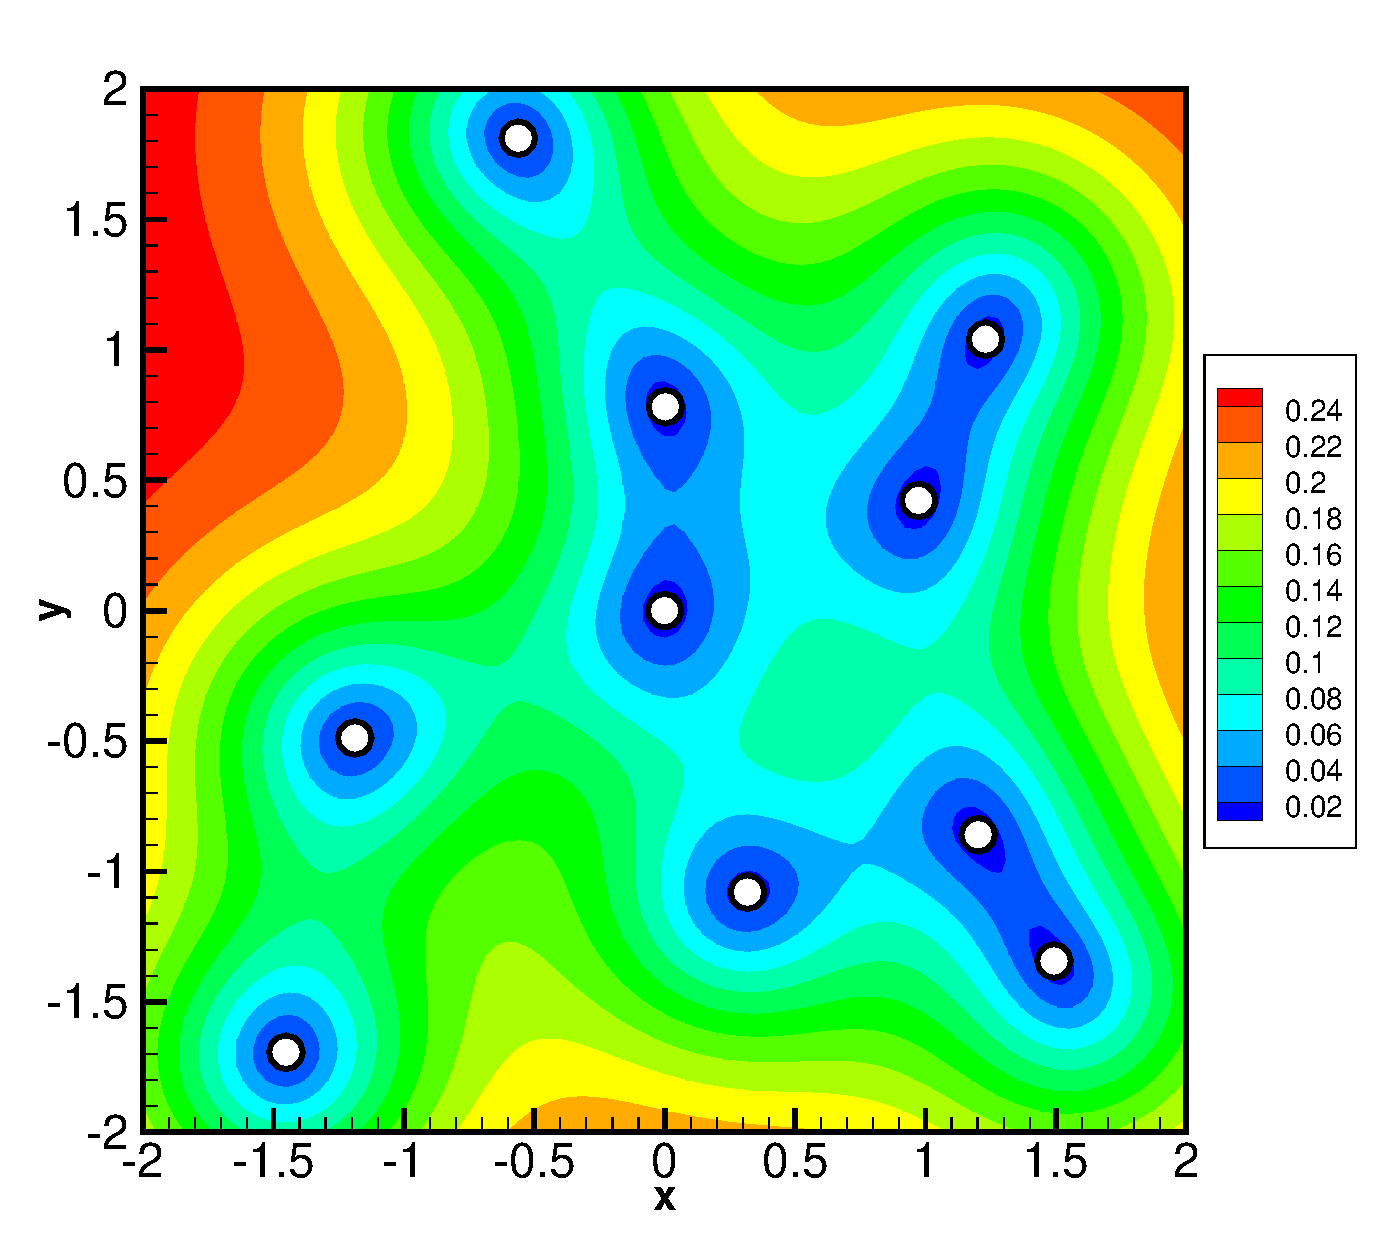
\includegraphics[width=1.0\textwidth]{figures/mse10runge.eps}\subcaption{N=10}
\end{minipage}
\begin{minipage}[b]{0.48\linewidth}
   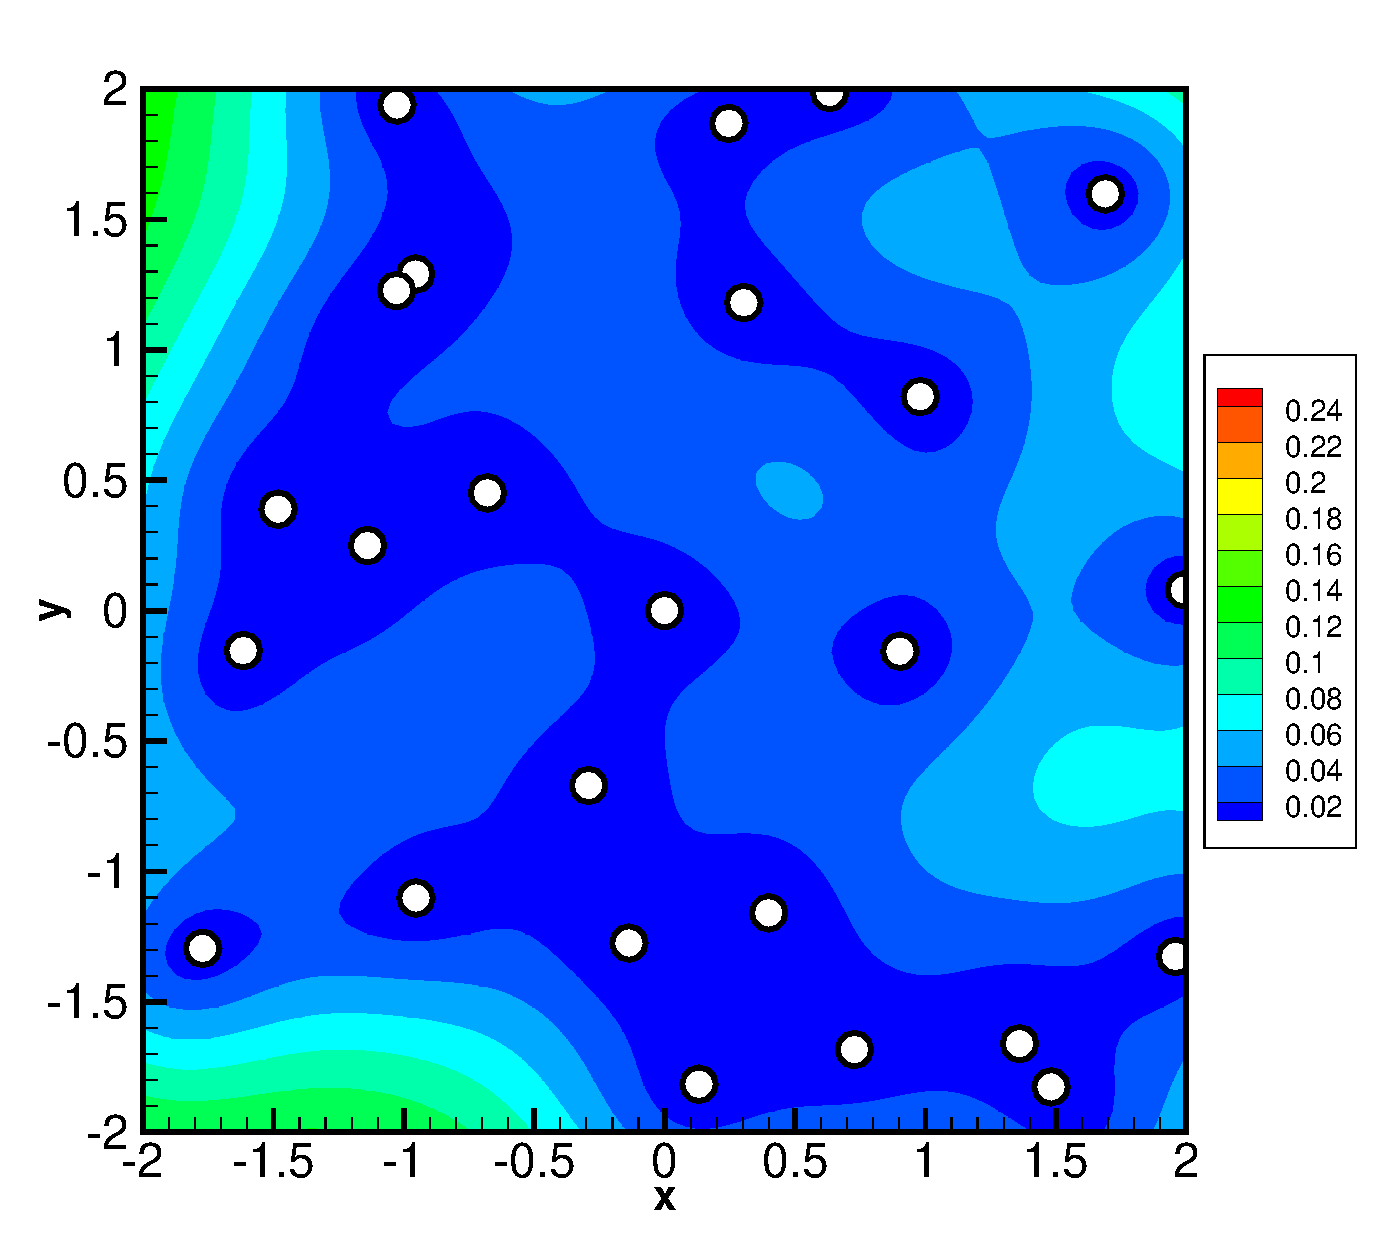
\includegraphics[width=1.0\textwidth]{figures/mse25runge.eps}\subcaption{N=25}
\end{minipage}
\caption[An example of mean squared error estimate provided by kriging.]{An example of MSE estimate provided by kriging using two-dimensional Runge function. The white circles refer to training point locations.}
\label{fig:MSErunge}
\end{figure}

\subsubsection*{Expected Improvement}

Jones~\etal~\cite{Jones98} suggested that training points can be selected in regions where the \emph{expected improvement} (EI) function defined by Eq.~\ref{eq:EI} is maximal, \emph{i.e.} in regions where the expectation of improvement in the objective function is maximal. During this process, the training point set is updated, the metamodel is reconstructed, and the process of choosing additional training points is continued until the expected improvement from a potential new training point has become sufficiently small. 

The EI based training point selection approach has great potential for finding the global optimum. However, this approach assumes MSE to be the actual error in the kriging prediction, when it is indeed  not, and regions near the current best point have a greater EI value, causing the algorithm to cluster points near the current best point. Figure~\ref{fig:EIrunge} shows the contours of the EI function over the domain of a two-dimensional Runge function.

\begin{figure}[h!]
\centering
\begin{minipage}[b]{0.48\linewidth}
   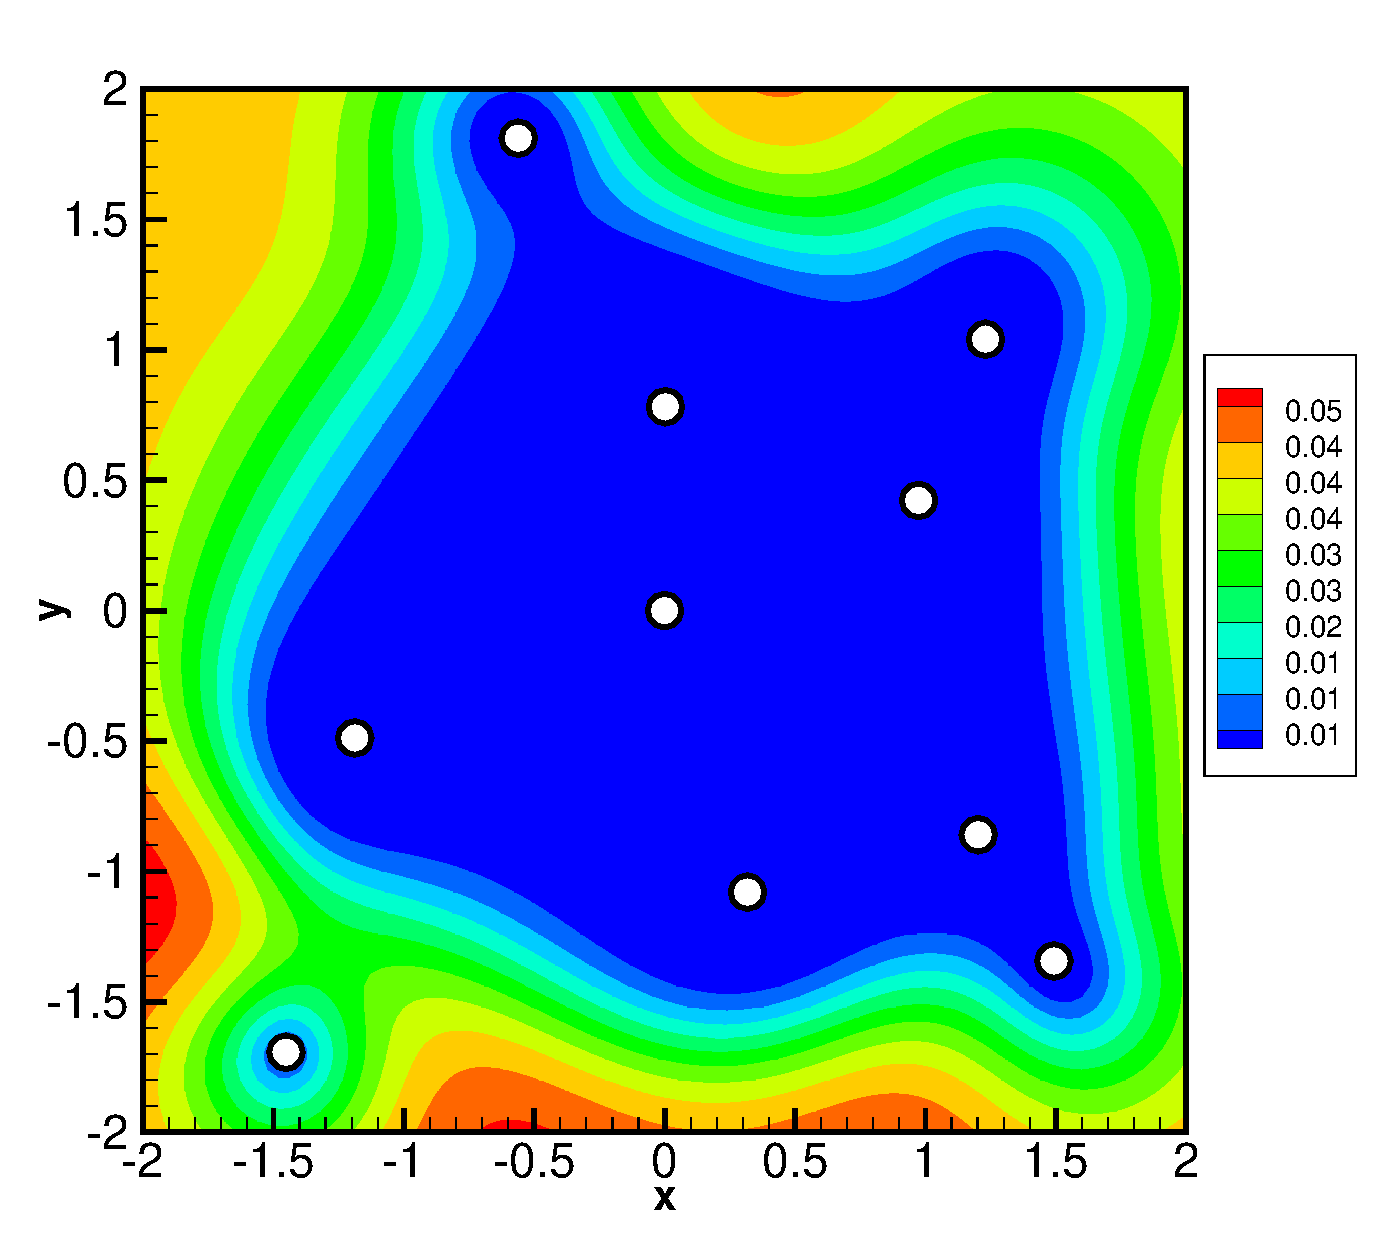
\includegraphics[width=1.0\textwidth]{figures/EI10runge.eps}\subcaption{N=10}
\end{minipage}
\begin{minipage}[b]{0.48\linewidth}
   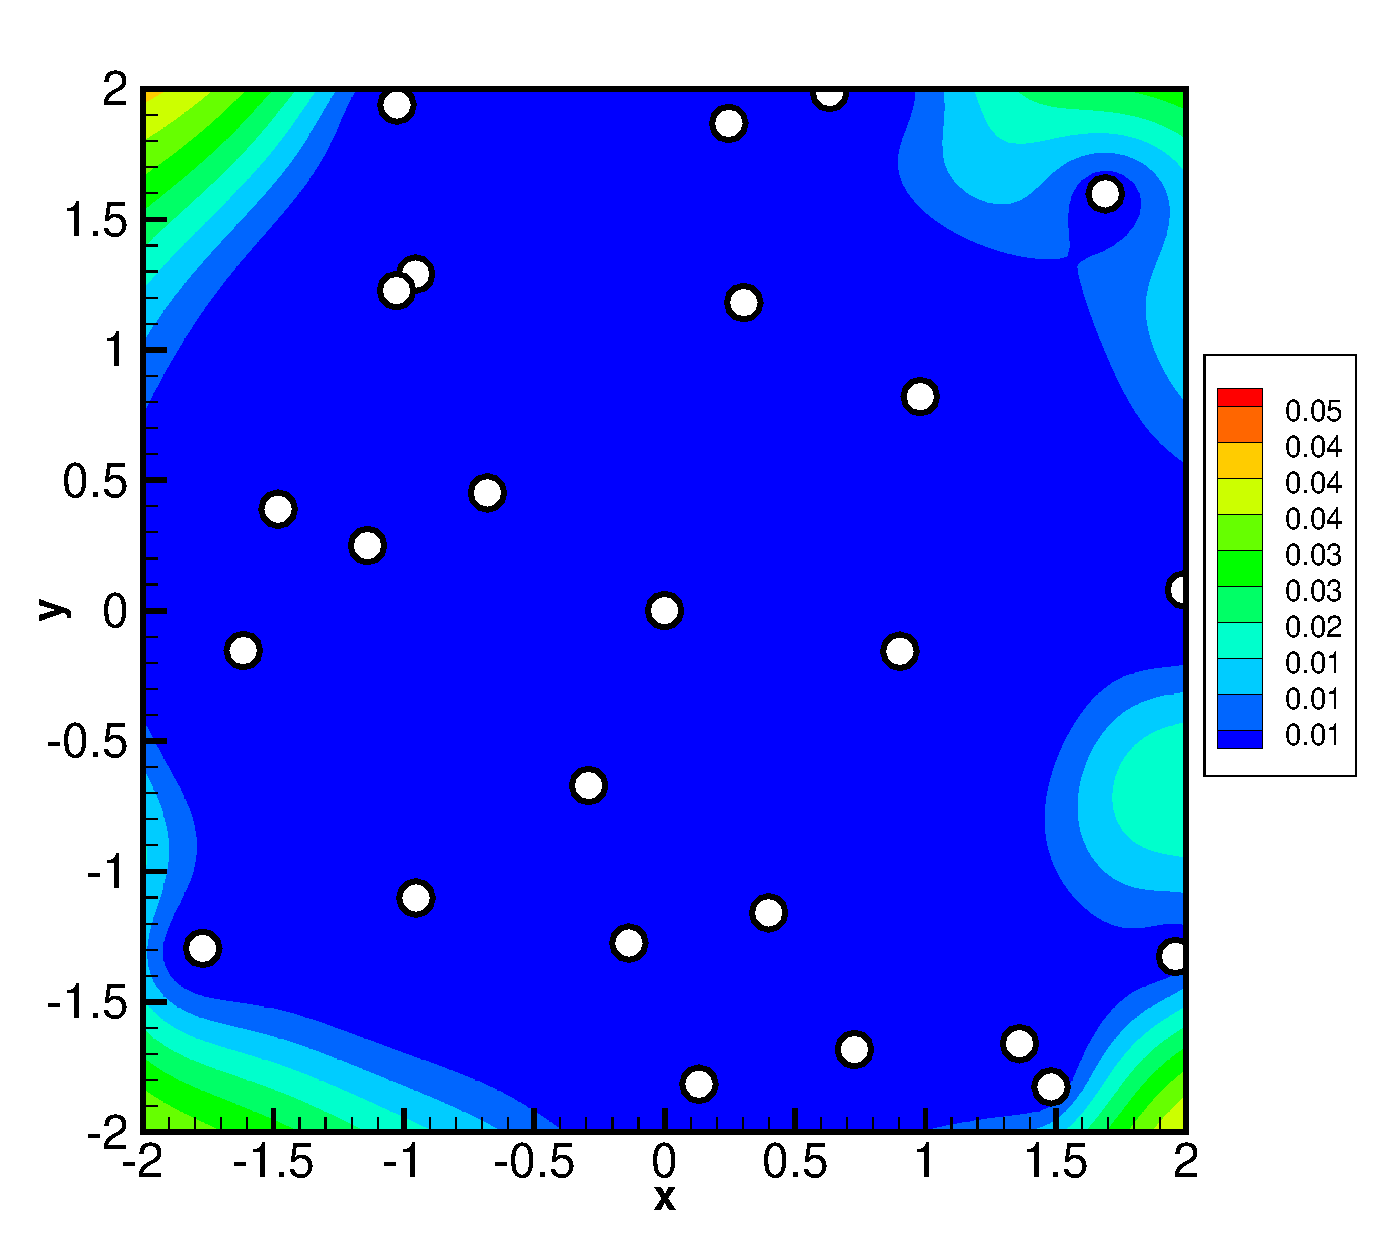
\includegraphics[width=1.0\textwidth]{figures/EI25runge.eps}\subcaption{N=25}
\end{minipage}
\caption[An example of expected improvement estimate provided by kriging]{Expected improvement provided by kriging using two-dimensional Runge function. The white circles refer to training point locations.}
\label{fig:EIrunge}
\end{figure}

%\subsubsection*{Demerits}
Though MSE/EI can be a better option than random training point selection, the methods have some disadvantages that are summarized below:
\begin{itemize}
\item MSE formulation does not incorporate any information from the actual response values $f(\x)$.
\item Not all surrogate modeling approaches provide MSE/EI estimates like kriging.
\item Even though kriging has an MSE estimate, mathematically it is not an actual measure of error in the kriging prediction.
\item EI is much more suited for optimization rather than building a globally accurate surrogate model as required for UQ.
\end{itemize}




% Since the Kriging method is known to have a good interpolation
%but a weak extrapolation quality this behavior seems reasonable. When aiming at a good global approximation quality in
%a (convex) constrained domain, one has to assure that every point of the domain is surrounded by neighboring samples.
%That is to say even points close to the boundaries can be described as a convex-combination of adjacent samples, which is guaranteed by adding sufficient samples on the boundary. Adjacent now is regarded in terms of the correlation R(x−xj , θ), see (8). The cl , cd , cm responses are strongly correlated along the α-axis but only weakly correlated along the Ma-axis 1 (θ1 θ2), so adding more samples to the boundaries than to the Ma-boundaries seems reasonable. This results in 1 outperforming average LHC samplings, even if the MSE formulation (24) does not incorporate any information of the
%response y(xi ) directly.

\subsection{Trust Region Method}

The trust region method is associated  with an approximation to the exact function which is only ``trusted'' within a small region of the current optimization iterate. 
The size of the trust region is modified during the search, based on how well the model agrees with actual function evaluations. If the approximation is in good agreement the trust region is expanded and it is contracted if the approximation is determined to be poor. 
Alexandrov~\etal~\cite{Alexandrov98} proposed a \emph{metamodel management framework} using trust region method for updating the metamodels (adding training data) according to improvements in the objective function during an optimization procedure. 
